%set the master document for easy compilation
%!TEX root = ../D3_5_2.tex

\section{Manage\_Track\_Data}

\subsection{Component Requirements}

\begin{longtable}{p{.25\textwidth}p{.7\textwidth}}
\toprule
Component name			& Manage\_Track\_Data \\
\midrule
Link to SCADE model		& {\footnotesize \url{???}} \\
\midrule
SCADE designer			& ??? \\
\midrule
Description				& ??? \\
\midrule
Input documents	& 
Subset-026, Chapter ???\\
\midrule
Safety integrity level		& 4 \\
\midrule
Time constraints		& [If applicable description of time constraints, otherwise n/a] \\
\midrule
API requirements 		& [If applicable description of API requirements, otherwise n/a] \\
\bottomrule
\end{longtable}


\subsection{Interface}

An overview of the interface of component [component name] is shown in Figure~\ref{f:manage_track_data}. The inputs and outputs are described in detail in Section~\ref{s:manage_track_data_inputs} respectively \ref{s:manage_track_data_outputs}.

\begin{figure}
\center
{[Put SysML diagram of component here]}
\caption{Component SysML diagram}\label{f:manage_track_data_interface}
\end{figure}


\subsubsection{Inputs}\label{s:manage_track_data_inputs}

\paragraph{[Input 1 name]}

\begin{longtable}{p{.25\textwidth}p{.7\textwidth}}
\toprule
Input name				& [Name of the input] \\
\midrule
Description				& [Brief description of the input] \\
\midrule
Source					& [Name of the source component] \\ 
\midrule
Type					& [Type of the input] \\
\midrule
Valid range of values	& [Complete list of valid values] \\
\midrule
Behaviour when value is at boundary	& [Description of components behaviour when input value is at boundary] \\
\midrule
Behaviour for values out of valid range	& [Description of components behaviour when input value is out of valid range] \\
\bottomrule
\end{longtable}


\paragraph{[Input 2 name]}

\begin{longtable}{p{.25\textwidth}p{.7\textwidth}}
\toprule
Input name				& [Name of the input] \\
\midrule
Description				& [Brief description of the input] \\
\midrule
Source					& [Name of the source component] \\ 
\midrule
Type					& [Type of the input] \\
\midrule
Valid range of values	& [Complete list of valid values] \\
\midrule
Behaviour when value is at boundary	& [Description of components behaviour when input value is at boundary] \\
\midrule
Behaviour for values out of valid range	& [Description of components behaviour when input value is out of valid range] \\
\bottomrule
\end{longtable}


\subsubsection{Outputs}\label{s:manage_track_data_inputs}

\paragraph{[Output 1 name]}

\begin{longtable}{p{.25\textwidth}p{.7\textwidth}}
\toprule
Output name				& [Name of the output] \\
\midrule
Description				& [Brief description of the output] \\
\midrule
Destination				& [Name of the destination component(s)] \\ 
\midrule
Type					& [Type of the output] \\
\midrule
Valid range of values	& [Complete list of valid values] \\
\midrule
Behaviour when value is at boundary	& [Description of components behaviour when output value is at boundary] \\
\midrule
Behaviour for values out of valid range	& [Description of components behaviour when output value is out of valid range] \\
\bottomrule
\end{longtable}


\paragraph{[Output 2 name]}

\begin{longtable}{p{.25\textwidth}p{.7\textwidth}}
\toprule
Output name				& [Name of the output] \\
\midrule
Description				& [Brief description of the output] \\
\midrule
Destination				& [Name of the destination component(s)] \\ 
\midrule
Type					& [Type of the output] \\
\midrule
Valid range of values	& [Complete list of valid values] \\
\midrule
Behaviour when value is at boundary	& [Description of components behaviour when output value is at boundary] \\
\midrule
Behaviour for values out of valid range	& [Description of components behaviour when output value is out of valid range] \\
\bottomrule
\end{longtable}


\subsection{Sub Components}

\subsubsection{Calculate\_Train\_Position}
%set the master document for easy compilation
%!TEX root = ../D3_5_3.tex

\paragraph{Component Requirements}

\begin{longtable}{p{.25\textwidth}p{.7\textwidth}}
\toprule
Component name			& calculateTrainPosition \\
\midrule
Link to SCADE model		& {\footnotesize \url{https://github.com/openETCS/modeling/tree/master/model/Scade/System/ObuFunctions/ManageLocationRelatedInformation/TrainPosition/CalculateTrainPosition}} \\
\midrule
SCADE designer			& Uwe Steinke / Siemens AG \\
\midrule
Description				& The main purpose of the function is to calculate the locations of linked and unlinked balise groups (BGs) and the current train position while the train is running along the track. In detail, the calculateTrainPosition function provides a couple of essential subfunctions for the onboard unit. These are mainly
\begin{itemize}
\item creating and maintaining an obu internal coordinate system for all types of location based data
\item storing all linked and unlinked balise groups resulting from over passing or from announcements (linking information) from the track
\item calculating and maintaining the locations of all stored balise groups during the train trip, based on odometry and linking information
\item permanently calculating the current train position based on odometry and passed balise group information
\item providing the last recently passed linked balise group as the LRBG
\item providing additional position attribute information
\item deleting stored balise groups, when appropriate
\item detecting linking consistency errors
\item determining, if linking is used on board
\end{itemize}
The calculation algorithms for locations and positions are implemented as specified in 
{\footnotesize\url{https://github.com/openETCS/SRS-Analysis/blob/master/System%20Analysis/WorkingRepository/Group4/SUBSET_26_3-6/DetermineTrainLocationProcedures.pdf}} \\
\midrule
Input documents	& 
Subset-026, Chapter 3.6 \\
\midrule
Safety integrity level		& 4 \\
\midrule
Time constraints		& n/a \\
\midrule
API requirements 		& Cf.~interface description of parent component. \\
\bottomrule
\end{longtable}


\paragraph{Interface}

For an overview of the interface of this internal component we refer to the SCADE model (cf.~link above) respectively the SCADE generated documentation.

%An overview of the interface of component calculateTrainPosition is shown in Figure~\ref{f:calculateTrainPosition_interface}. The inputs and outputs are described in detail in Section~\ref{s:calculateTrainPosition_inputs} respectively \ref{s:calculateTrainPosition_outputs}.
%
%\begin{figure}
%\center
%\missingfigure{[Put SysML diagram of component here]}
%\caption{Component SysML diagram}\label{f:calculateTrainPosition_interface}
%\end{figure}
%
%\subsubsection{Inputs}\label{s:calculateTrainPosition_inputs}
%
%\paragraph{currentOdometry}
%
%\begin{longtable}{p{.25\textwidth}p{.7\textwidth}}
%\toprule
%Input name				& currentOdometry \\
%
%\midrule
%Description				& currentOdometry is the actual odometry information as known by the whole EVC model and provided by the models external interface. \newline
%  \\
%\midrule
%Source					& External model interface input \\ 
%\midrule
%Type					& Obu\_BasicTypes\_Pkg::odometry\_T \\  
%\midrule
%Valid range of values	& Obu\_BasicTypes\_Pkg::odometry\_T is a complex data type. \\
%\midrule
%Valid range of values	& Obu\_BasicTypes\_Pkg::odometry\_T is a complex data type. Values are given for each element.\newline Format is: Type Name: range/ list of values
%\begin{itemize}
%\item bool valid: [true | false]. Must be permanently set to "true".
%\item timestamp: (0 - 2147483647). Current time in ms, must be monotonically increasing.
%\item odo: Obu\_BasicTypes\_Pkg::OdometryLocations\_T: current odometry log values with uncertainties; must behave according to {\footnotesize\url{https://github.com/openETCS/SRS-Analysis/blob/master/System%20Analysis/WorkingRepository/Group4/SUBSET_26_3-6/DetermineTrainLocationProcedures.pdf}} [[ 3.1 ]]. Members of OdometryLocations\_T are: 
%\begin{itemize}
%\item o\_nominal: L\_internal\_Type: nominal value in cm.
%\item o\_min:     L\_internal\_Type: \newline min. distance = o\_min2 - o\_min1
%\item o\_max:     L\_internal\_Type: \newline max distance = o\_max2 - o\_max1
%\end{itemize}
%
%\item speed: Obu\_BasicTypes\_Pkg::OdometrySpeeds\_T: not used by calculateTrainPosition
%\item acceleration: Obu\_BasicTypes\_Pkg::A\_internal\_Type: not used by calculateTrainPosition
%\item motionState: \newline [noMotion | Motion]
%\item motionDirection: Obu\_BasicTypes\_Pkg::odoMotionDirection\_T \newline [ unknownDirection | cabAFirst | cabBFirst ]
%\end{itemize}  \\
%
%                     	&  \emph{calculateTrainPosition requires consistent value sets of currentOdometry. calculateTrainPosition itself does not check.}
%\\
%
%\midrule
%Behaviour when value is at boundary	& n/a \\
%\midrule
%Behaviour for values out of valid range	& Enumerated values out of range prohibit code generation. In all other cases, calculateTrainPosition does not have the knowledge for out-of-range checks. \\
%\bottomrule
%\end{longtable}
%
%
%
%\paragraph{msgFromTrack}
%
%\begin{longtable}{p{.25\textwidth}p{.7\textwidth}}
%\toprule
%Input name				& msgFromTrack \\
%
%\midrule
%Description				& With msgFromTrack calculateTrainPosition receives datagrams from balise groups and RBC. \newline
%  \\
%\midrule
%Source					& Manage\_TrackSideInformation\_Integration\_Pkg::Manage\_TrackSideInformation\_Integration/ \\ 
%\midrule
%Type					& Common\_Types\_Pkg::ReceivedMessage\_T \\  
%\midrule
%Valid range of values	& Common\_Types\_Pkg::ReceivedMessage\_T is a complex data type. Values are given for each element.\newline Format is: Type Name: range/ list of values
%\begin{itemize}
%\item bool valid: [true | false]. "true" flags a datagram as received and to be evaluated by calculateTrainPosition. Must be set for exactly 1 clock for each received datagram and stay unset otherwise
%\item source: Common\_Types\_Pkg::MsgSource\_T: Designates the source of the datagram: \newline ( msrc\_undefined | msrc\_Euroradio | msrc\_Eurobalise | msrc\_RadioInfillUnit | msrc\_OBU ) 
%
%\item radioMetaData: Common\_Types\_Pkg::radioMetaData\_T: not used by calculateTrainPosition
%
%\item BG\_Common\_Header: BG\_Types\_Pkg::BG\_Header\_T: Header information received from balise groups, refer to Manage\_TrackSideInformation\_Integration\_Pkg::Manage\_TrackSideInformation\_Integration
%
%\item Radio\_Common\_Header: Radio\_Types\_Pkg::Radio\_TrackTrain\_Header\_T: Header information received from RBC via radio, refer to Manage\_TrackSideInformation\_Integration\_Pkg::Manage\_TrackSideInformation\_Integration
%
%\item packets: Common\_Types\_Types\_Pkg::CompressedPackets\_T: datagram packets, refer to Manage\_TrackSideInformation\_Integration\_Pkg::Manage\_TrackSideInformation\_Integration. calculatesTrainPosition extracts packet 5 (linking information), if available.
%
%\item sendingRBC: Common\_Types\_Types\_Pkg::RBC\_Id\_T: designates the origin RBC and the mobile modem channel used onboard, if received via radio. Refer to Manage\_TrackSideInformation\_Integration\_Pkg::Manage\_TrackSideInformation\_Integration for more detailed information.
%
%\end{itemize}  \\
%
%                     	&  \emph{calculateTrainPosition expects the received information to be consistent and validated before applied to. It does not check, if the information is appropriate due to current EVC mode, level, train or balise orientation. Received balise group or linking information already known by calculateTrainPosition overrides former data.}
%\\
%
%\midrule
%Behaviour when value is at boundary	& n/a \\
%\midrule
%Behaviour for values out of valid range	& Enumerated values out of range prohibit code generation. In all other cases, calculateTrainPosition does not have the knowledge for out-of-range checks. \\
%
%\bottomrule
%\end{longtable}
%
%
%
%
%\paragraph{trainProperties}
%
%\begin{longtable}{p{.25\textwidth}p{.7\textwidth}}
%\toprule
%Input name				& trainProperties \\
%
%\midrule
%Description				& Supplies calculateTrainPosition with train specific properties required for position calculation. \newline
%  \\
%\midrule
%Source					& EVC\_Support\_Pkg::maintainTrainProperties/ \\ 
%\midrule
%Type					& TrainPosition\_Types\_Pck::trainProperties\_T \\  
%\midrule
%Valid range of values	& TrainPosition\_Types\_Pck::trainProperties\_T is a complex data type. Values are given for each element.\newline Format is: Type Name: range/ list of values
%\begin{itemize}
%\item nid\_engine:: NID\_ENGINE as defined by subset 026-7. 
%\item nid\_operational: NID\_OPERATIONAL as defined by subset 026-7. 
%\item l\_train: L\_TRAIN as defined by subset 026-7. 
%
%\item d\_baliseAntenna\_2\_frontend: Obu\_BasicTypes\_Pkg::LocWithInAcc\_T:  Distance from the trains balise antenna to the trains front end, in cm with uncertainties. 
%
%\item d\_frontend\_2\_rearend: Obu\_BasicTypes\_Pkg::LocWithInAcc\_T:  Distance from the trains Distance from the trains front end to rear end, in cm with uncertainties. 
%
%\item locationAccuracy\_DefaultValue: Obu\_BasicTypes\_Pkg::LocWithInAcc\_T:  Default location accuracy of balise groups (subset 026, 3.6.4.3.2), in cm with uncertainties. 
%
%\item centerDetectionAcc\_DefaultValue: Obu\_BasicTypes\_Pkg::LocWithInAcc\_T:  Default  accuracy of balise groups detection of the BTM, in cm with uncertainties. Will be applied, if centerDetectionInaccuracy from BTM is not available, especially for announced and not yet passed BGs. 
%
%\end{itemize}  \\
%
%                     	&  \emph{calculateTrainPosition expects this information to be consistent and validated before applied to.}
%\\
%
%\midrule
%Behaviour when value is at boundary	& n/a \\
%\midrule
%Behaviour for values out of valid range	& Enumerated values out of range prohibit code generation. In all other cases, calculateTrainPosition does not have the knowledge for out-of-range checks. \\
%
%\bottomrule
%\end{longtable}
%
%
%
%\paragraph{passedBG}
%
%\begin{longtable}{p{.25\textwidth}p{.7\textwidth}}
%\toprule
%Input name				& passedBG \\
%
%\midrule
%Description				& Deprecated alternative input to msgFromTrack. Must not be used any more and is subject to be removed in subsequent releases.  \newline
%  \\
%
%\bottomrule
%\end{longtable}
%
%
%\paragraph{reset}
%
%\begin{longtable}{p{.25\textwidth}p{.7\textwidth}}
%\toprule
%Input name				& reset \\
%
%\midrule
%Description				& Resets and keeps calculateTrainPosition at its initial state and deletes all internally stored data. \newline
%  \\
%\midrule
%Source					& To whom it may concern/ \\ 
%\midrule
%Type					& bool \\  
%\midrule
%Valid range of values	& [ false | true ] \\
%
%\midrule
%Behaviour when value is at boundary	& n/a \\
%\midrule
%Behaviour for values out of valid range	& Enumerated values out of range prohibit code generation. \\
%
%\bottomrule
%\end{longtable}
%
%
%\subsubsection{Outputs}\label{s:calculateTrainPosition_outputs}
%
%\paragraph{trainPosition}
%
%\begin{longtable}{p{.25\textwidth}p{.7\textwidth}}
%\toprule
%Output name				& trainPosition \\
%
%\midrule
%Description				& Provides the current train position and LRBG with its attributes. All distance and location computations of the OBU must be based on this information. \newline
%  \\
%\midrule
%Destination				& Any drain component which needs the current train position or  LRBG \\ 
%\midrule
%Type					& TrainPosition\_Types\_Pck::trainPosition\_T \\  
%\midrule
%Valid range of values	& TrainPosition\_Types\_Pck::trainPosition\_T is a complex data type. Values are given for each element.\newline Format is: Type Name: range/ list of values
%\begin{itemize}
%\item valid: bool: [true | false]. Always true, except for exceptional circumstances.
%\item timestamp: Obu\_BasicTypes\_Pkg::T\_internal\_Type: latest time in ms. 
%\item trainPositionIsUnknown: bool: true, if the train position is evaluated as "unknonwn" (refer to subset-026, 3.6.3.1.3.1). 
%\item noCoordinateSystemHasBeenAssigned: bool: refer to subset 026, 3.4.2, 3.6.3.1.4
%\item trainPosition: Obu\_BasicTypes\_Pkg::LocWithInAcc\_T: The calculated train position with uncertainties
%\item estimatedFrontEndPosition: Obu\_BasicTypes\_Pkg::Location\_T: Train front end position in cm.
%\item minSafeFrontEndPosition: Obu\_BasicTypes\_Pkg::Location\_T: Train front end position in cm.
%\item maxSafeFrontEndPostion: Obu\_BasicTypes\_Pkg::Location\_T: Train front end position in cm.
%\item LRBG: TrainPosition\_Types\_Pck::positionedBG\_T: the current LRBG. 
%\item prvLRBG: TrainPosition\_Types\_Pck::positionedBG\_T: the balise group passed previously to LRBG. For type definition, see below.
%\item nominalOrReverseToLRBG: Q\_DLRBG: Orientation of the train in relation to the direction of the LRBG, see subset 026-7.
%\item trainOrientationToLRBG: Q\_DIRLRBG: Orientation of the train in relation to the direction of the LRBG, see subset 026-7.
%\item trainRunningDirectionToLRBG: Q\_DIRTRAIN: Direction of train movement in relation to the LRBG orientation, see subset 026-7.
%\item linkingIsUsedOnboard: bool: Designates, if at least one announced linked BG is ahead
%
%\end{itemize}  \\
%
%                     	&  \emph{calculateTrainPosition provides the train position to whom it concerns and recalculates it with every clock cycle}
%\\
%
%\midrule
%Behaviour when value is at boundary	& n/a \\
%\midrule
%Behaviour for values out of valid range	& n/a \\
%
%\midrule
%Behaviour when value is errorneous, absent or unwanted & n/a \\
%
%\bottomrule
%\end{longtable}
%
%
%\paragraph{BGs}
%
%\begin{longtable}{p{.25\textwidth}p{.7\textwidth}}
%\toprule
%Output name				& BGs \\
%
%\midrule
%Description				& A list of all linked and unlinked balise groups - known to calculateTrainPosition - in the order they are arranged on the track.  \newline
%  \\
%\midrule
%Destination				& Any subsequent component which needs the current collection of balises groups \\ 
%\midrule
%Type					& array of TrainPosition\_Types\_Pck::positionedBG\_T \\  
%\midrule
%Valid range of values	& TrainPosition\_Types\_Pck::positionedBG\_T is a complex data type. Values are given for each array element.\newline Format is: Type Name: range/ list of values
%\begin{itemize}
%\item valid: bool: [true | false]. "true" for every existing balise group.
%\item nid\_c: NID\_C: refer to subset 026-7. 
%\item nid\_bg: NID\_BG: refer to subset 026-7. 
%\item q\_link: Q\_LINK: refer to subset 026-7. 
%\item location: Obu\_BasicTypes\_Pkg::LocWithInAcc\_T: The best known location (with inaccuracies) calculated from linking and from passing information.
%\item seqNoOnTrack: int: Sequence number, specifies the order of the BG passed or expected to be passed
%\item infoFromLinking: TrainPosition\_Types\_Pck::infoFromLinking\_T: Describes a linked BG as announced from the linking BG. Mainly, this information is taken from the linking packet.
%\item infoFromPassing: BG\_Types\_Pkg::passedBG\_T: If the balise group has been passed already, this is the relevant information received from the BG.
%
%\end{itemize}  \\
%
%                     	&  \emph{calculateTrainPosition provides the list of balise groups to whom it concerns.}
%\\
%
%\midrule
%Behaviour when value is at boundary	& n/a \\
%\midrule
%Behaviour for values out of valid range	& n/a \\
%
%\midrule
%Behaviour when value is errorneous, absent or unwanted & n/a \\
%
%\bottomrule
%\end{longtable}
%
%\paragraph{errors}
%
%\begin{longtable}{p{.25\textwidth}p{.7\textwidth}}
%\toprule
%Output name				& errors \\
%
%\midrule
%Description				& Provides a collection of error flags, raised by calculateTrainPosition.  \newline
%  \\
%\midrule
%Destination				& Error handlers and components which need to know of common and linking consistency errors.  \\ 
%\midrule
%Type					& TrainPosition\_Types\_Pck::positionErrors\_T \\  
%\midrule
%Valid range of values	& TrainPosition\_Types\_Pck::positionErrors\_T is a complex data type. Values are given for each array element.\newline Format is: Type Name: range/ list of values
%\begin{itemize}
%\item outOfMemSpace: bool: Memory overrun: a passed or announced BG could not be stored.
%\item passedBG\_foundNotWhereExpected: bool: The currently passed linked BG location does not match its expectation window.
%\item positionCalculation\_inconsistent: A consistency problem arose during position calculation.
%\item linkedBGMissed: bool: The expectation window for an announced BG was passed without detecting the BG.
%\item BGpassedInUnexpectedDirection: bool: The BG was passed in a different orientation than announced via linking.
%\item BG\_LinkingConsistencyError: bool: Linking consistency error (ref. subset 026, 3.16.2.3).
%\item twoConsecutiveLinkedBGs\_missed: bool: 2 consecutive linked balise groups announced by linking are not detected and the end of the expectation window of the second balise group has been passed (subset 026, 3.16.2.7.1).
%\item doubleRepositioningError: bool: Double repositioning error (3.16.2.7.2).
%\item bg: TrainPosition\_Types\_Pck::positionedBG\_T: The corresponding balise group in the case of an error.
%
%\end{itemize}  \\
%
%\midrule
%Behaviour when value is at boundary	& n/a \\
%\midrule
%Behaviour for values out of valid range	& n/a \\
%
%\midrule
%Behaviour when value is errorneous, absent or unwanted & n/a \\
%
%\bottomrule
%\end{longtable}
%


\subsubsection{Provide\_Position\_Report}
%set the master document for easy compilation
%!TEX root = ../D3_5_3.tex

\section{F2.8: Provide\_Position\_Report}

\subsection{Component Requirements}

\begin{longtable}{p{.25\textwidth}p{.7\textwidth}}
\toprule
Component name			& Provide\_Position\_Report \\
\midrule
Link to SCADE model		& {\footnotesize \url{https://github.com/openETCS/modeling/blob/master/model/Scade/System/ObuFunctions/ManageLocationRelatedInformation/TrainPosition/ProvidePositionReport/ProvidePositionReport_Pkg.xscade}}\\
\midrule
SCADE designer			& Christian Stahl, TWT GmbH \\
\midrule
Description				& The component builds a position report for the RBC, i.e., message 132, and provides it as an output.  There are two triggers for sending message 132:  
\begin{enumerate}
\item at least one of the triggers of the position report parameters (packet 58) holds or 
\item one of the events enabling the sending of the report occurs.
\end{enumerate} 
As the core position report (i.e., packet 0 or 1) is included in other packets, the
component also provides this core position report at every clock cycle. At most one of the two packets is valid.\\
\midrule
Input documents	& 
Subset-026, Chapter 3.6.5 \\
\midrule
Safety integrity level		& 4 \\
\midrule
Time constraints		& n/a
\\
\midrule
API requirements 		& n/a \\
\bottomrule
\end{longtable}


\subsection{Interface}

An overview of the interface of component Provide\_Position\_Report is shown in Figure~\ref{f:provide_position_report_interface}. The inputs and outputs are described in detail in Section~\ref{s:provide_position_report_inputs} respectively \ref{s:provide_position_report_outputs}. Subcomponents are described in Section~\ref{s:provide_position_report_subcomponents}.

\begin{figure}
\center
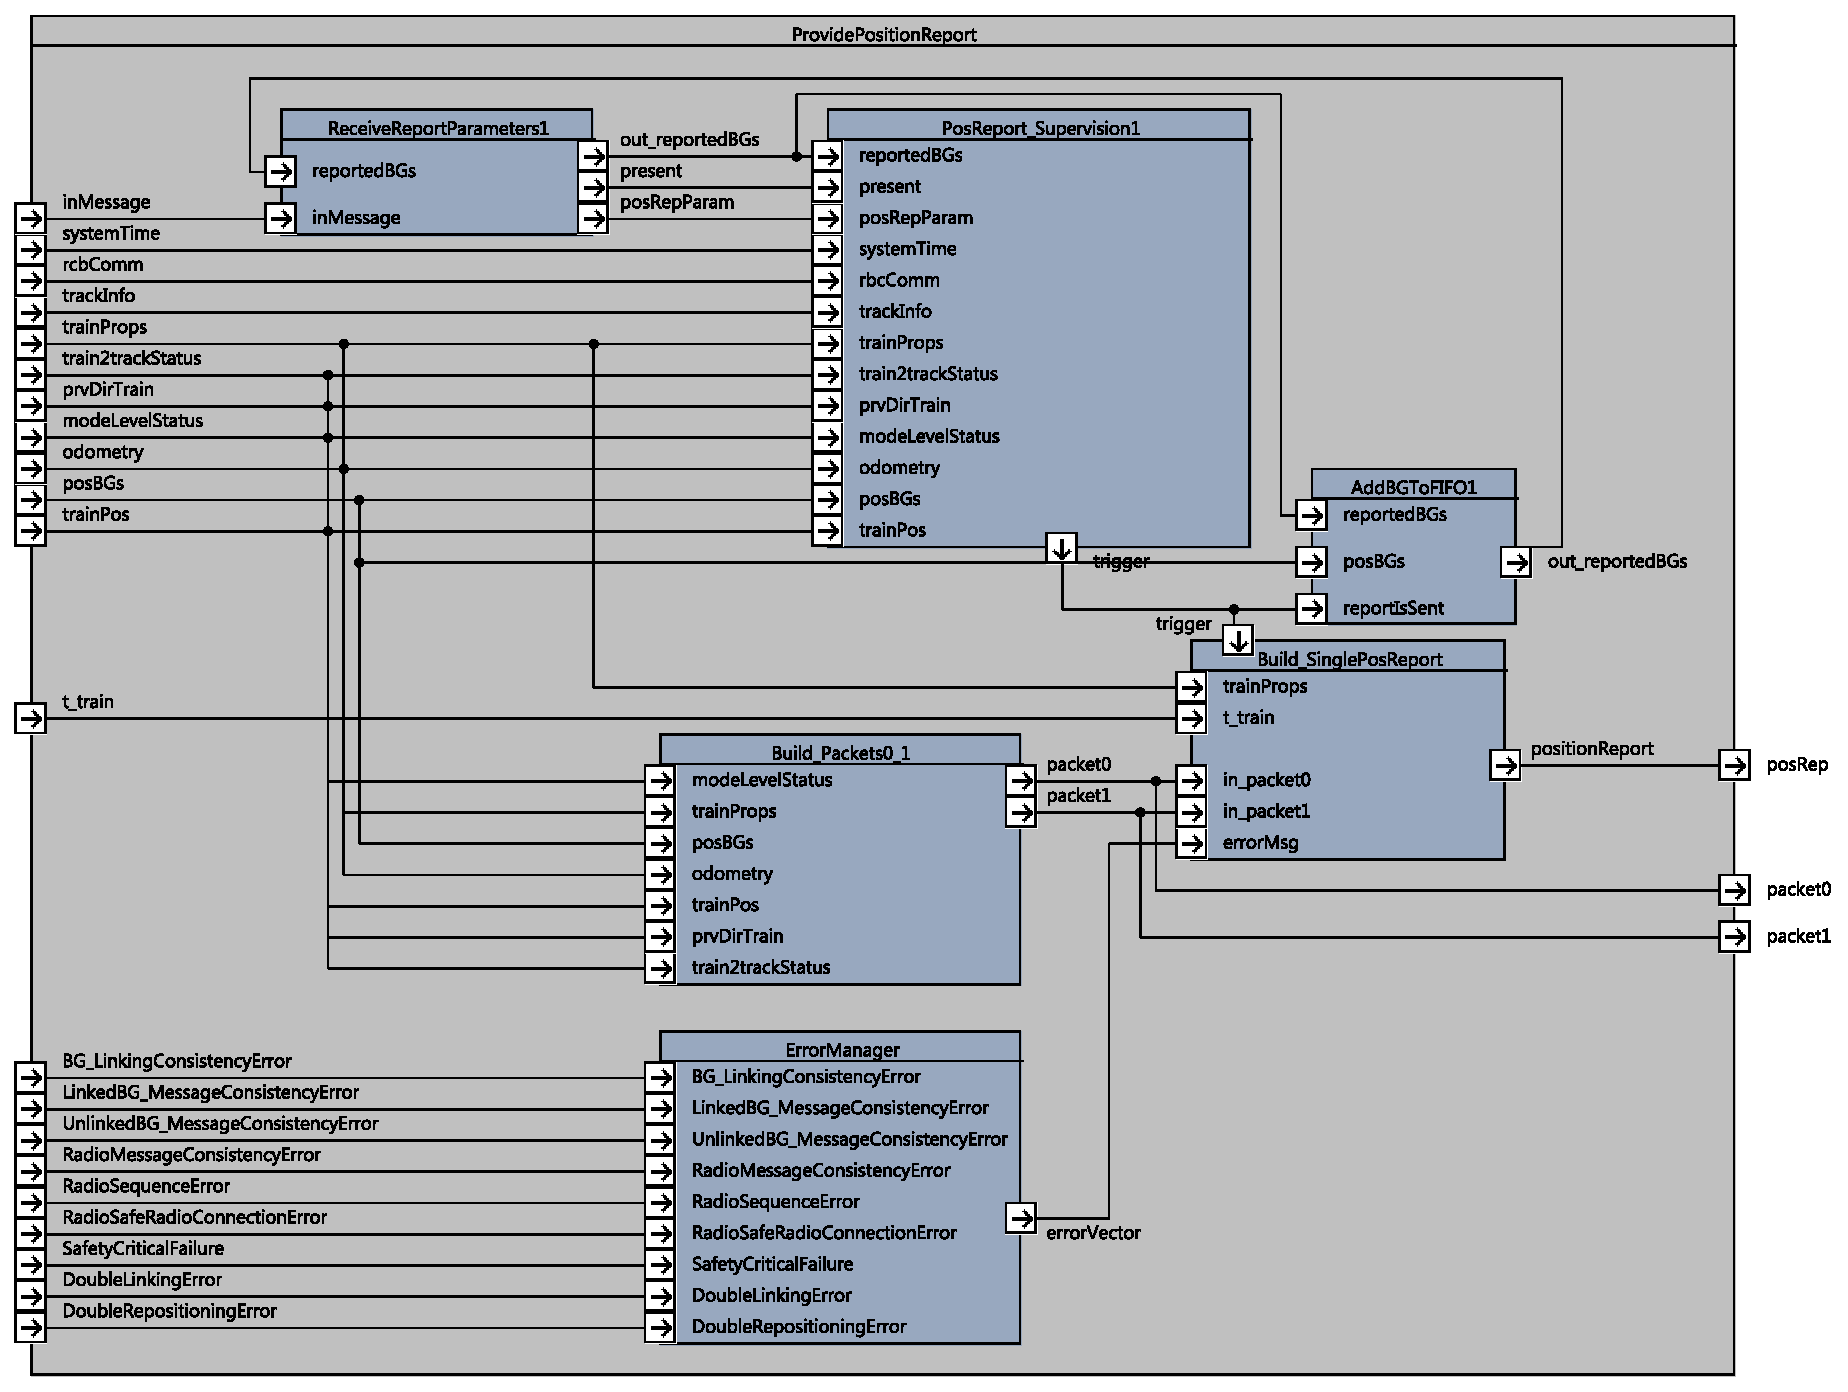
\includegraphics[width=\textwidth]{ProvidePositionReport_SysML}
\caption{Provide\_Position\_Report component SysML diagram}\label{f:provide_position_report_interface}
\end{figure}


\subsubsection{Inputs}\label{s:provide_position_report_inputs}

\paragraph{inMessage}

\begin{longtable}{p{.25\textwidth}p{.7\textwidth}}
\toprule
Input name				& inMessage \\
\midrule
Description				& Input message from the bus (to extract Packet 58, the position report parameters). \\
\midrule
Source					& Manage\_TrackSideInformation\_Integration\_Pkg::\newline Manage\_TrackSideInformation\_Integration \\ 
\midrule
Type					& Common\_Types\_Pkg::ReceivedMessage\_T \\
\midrule
Valid range of values	& as defined in SCADE \\
\midrule
Behaviour when value is at boundary	& n/a \\
\midrule
Behaviour for values out of valid range	& n/a \\
\midrule
Behaviour when value is erroneous, absent or unwanted (i.e. spurious) & If valid is false, then input is ignored. \\
\bottomrule
\end{longtable}


\paragraph{systemTime}

\begin{longtable}{p{.25\textwidth}p{.7\textwidth}}
\toprule
Input name				& systemTime \\
\midrule
Description				& The system time. \\
\midrule
Source					& API \\ 
\midrule
Type					& SystemTime\_T, i.e., Obu\_BasicTypes\_Pkg::T\_internal\_Type \\
\midrule
Valid range of values	& [0; maximum positive int value of target platform] \\
\midrule
Behaviour when value is at boundary	& assumed to be valid \\
\midrule
Behaviour for values out of valid range	& assumed to be valid \\
\midrule
Behaviour when value is erroneous, absent or unwanted (i.e. spurious) & assumed to be valid \\
\bottomrule
\end{longtable}

\paragraph{rbcComm}

\begin{longtable}{p{.25\textwidth}p{.7\textwidth}}
\toprule
Input name				& rbcComm \\
\midrule
Description				& Variables modeling stati regarding the RBC communication. \\
\midrule
Source					& MoRC\_Pck::MoRC\_Main \\ 
\midrule
Type					& RBC\_Communication\_T \\
\midrule
Valid range of values	& as defined in SCADE \\
\midrule
Behaviour when value is at boundary	& n/a \\
\midrule
Behaviour for values out of valid range	& n/a \\
\midrule
Behaviour when value is erroneous, absent or unwanted (i.e. spurious) & n/a \\
\bottomrule
\end{longtable}

\paragraph{trackInfo}

\begin{longtable}{p{.25\textwidth}p{.7\textwidth}}
\toprule
Input name				& trackInfo \\
\midrule
Description				& Location based events. \\
\midrule
Source					& EVC; currently a constant \\ 
\midrule
Type					& LocationBasedEvents\_T \\
\midrule
Valid range of values	& as defined in SCADE \\
\midrule
Behaviour when value is at boundary	& n/a \\
\midrule
Behaviour for values out of valid range	& n/a \\
\midrule
Behaviour when value is erroneous, absent or unwanted (i.e. spurious) & n/a \\
\bottomrule
\end{longtable}

\paragraph{trainProps}

\begin{longtable}{p{.25\textwidth}p{.7\textwidth}}
\toprule
Input name				& trainProps \\
\midrule
Description				& The train properties. \\
\midrule
Source					& EVC\_Support\_Pkg::maintainTrainProperties \\ 
\midrule
Type					& TrainPosition\_Types\_Pck::trainProperties\_T \\
\midrule
Valid range of values	& as defined in SCADE \\
\midrule
Behaviour when value is at boundary	& n/a \\
\midrule
Behaviour for values out of valid range	& n/a \\
\midrule
Behaviour when value is erroneous, absent or unwanted (i.e. spurious) & n/a \\
\bottomrule
\end{longtable}

\paragraph{train2trackStatus}

\begin{longtable}{p{.25\textwidth}p{.7\textwidth}}
\toprule
Input name				& train2trackStatus \\
\midrule
Description				& Train to track status information. \\
\midrule
Source					& EVC \\ 
\midrule
Type					& BG\_Types\_Pkg::TrainToTrackStatus\_T \\
\midrule
Valid range of values	& as defined in SCADE \\
\midrule
Behaviour when value is at boundary	& n/a \\
\midrule
Behaviour for values out of valid range	& n/a \\
\midrule
Behaviour when value is erroneous, absent or unwanted (i.e. spurious) & n/a \\
\bottomrule
\end{longtable}

\paragraph{prvDirTrain}

\begin{longtable}{p{.25\textwidth}p{.7\textwidth}}
\toprule
Input name				& prvDirTrain \\
\midrule
Description				& Train direction of the last clock cycle. \\
\midrule
Source					& CalculateTrainPosition\_Pkg::calculateTrainPosition \\ 
\midrule
Type					& Q\_DIRTRAIN \\
\midrule
Valid range of values	& as defined in SCADE \\
\midrule
Behaviour when value is at boundary	& n/a \\
\midrule
Behaviour for values out of valid range	& n/a \\
\midrule
Behaviour when value is erroneous, absent or unwanted (i.e. spurious) & n/a \\
\bottomrule
\end{longtable}

\paragraph{modeLevelStatus}

\begin{longtable}{p{.25\textwidth}p{.7\textwidth}}
\toprule
Input name				& modeLevelStatus \\
\midrule
Description				& Information referring to mode and level status. \\
\midrule
Source					& ManageLevelAndMode \\ 
\midrule
Type					& ModeLevel2PositionReport\_T \\
\midrule
Valid range of values	& as defined in SCADE \\
\midrule
Behaviour when value is at boundary	& n/a \\
\midrule
Behaviour for values out of valid range	& n/a \\
\midrule
Behaviour when value is erroneous, absent or unwanted (i.e. spurious) & n/a \\
\bottomrule
\end{longtable}

\paragraph{odometry}

\begin{longtable}{p{.25\textwidth}p{.7\textwidth}}
\toprule
Input name				& odometry \\
\midrule
Description				& Odometry information.\\
\midrule
Source					& API \\ 
\midrule
Type					& Obu\_BasicTypes\_Pkg::odometry\_T \\
\midrule
Valid range of values	& as defined in SCADE \\
\midrule
Behaviour when value is at boundary	& n/a \\
\midrule
Behaviour for values out of valid range	& n/a \\
\midrule
Behaviour when value is erroneous, absent or unwanted (i.e. spurious) & n/a \\
\bottomrule
\end{longtable}

\paragraph{posBGs}

\begin{longtable}{p{.25\textwidth}p{.7\textwidth}}
\toprule
Input name				& posBGs \\
\midrule
Description				& Positioned balise groups used for current train position. \\
\midrule
Source					& CalculateTrainPosition\_Pkg::calculateTrainPosition \\ 
\midrule
Type					& TrainPosition\_Types\_Pck::positionedBGs\_T \\
\midrule
Valid range of values	& as defined in SCADE \\
\midrule
Behaviour when value is at boundary	& n/a \\
\midrule
Behaviour for values out of valid range	& n/a \\
\midrule
Behaviour when value is erroneous, absent or unwanted (i.e. spurious) & n/a \\
\bottomrule
\end{longtable}

\paragraph{trainPos}

\begin{longtable}{p{.25\textwidth}p{.7\textwidth}}
\toprule
Input name				& trainPos \\
\midrule
Description				& Current train position. \\
\midrule
Source					& CalculateTrainPosition\_Pkg::calculateTrainPosition \\ 
\midrule
Type					& TrainPosition\_Types\_Pck::trainPosition\_T \\
\midrule
Valid range of values	& as defined in SCADE \\
\midrule
Behaviour when value is at boundary	& n/a \\
\midrule
Behaviour for values out of valid range	& n/a \\
\midrule
Behaviour when value is erroneous, absent or unwanted (i.e. spurious) & n/a \\
\bottomrule
\end{longtable}

\paragraph{t\_train}

\begin{longtable}{p{.25\textwidth}p{.7\textwidth}}
\toprule
Input name				& t\_train \\
\midrule
Description				& Current timestamp. \\
\midrule
Source					& EVC \\ 
\midrule
Type					& T\_TRAIN \\
\midrule
Valid range of values	& as defined in SCADE \\
\midrule
Behaviour when value is at boundary	& n/a \\
\midrule
Behaviour for values out of valid range	& n/a \\
\midrule
Behaviour when value is erroneous, absent or unwanted (i.e. spurious) & n/a \\
\bottomrule
\end{longtable}

\paragraph{BG\_LinkingConsistencyError}

\begin{longtable}{p{.25\textwidth}p{.7\textwidth}}
\toprule
Input name				& BG\_LinkingConsistencyError \\
\midrule
Description				& True if respective error has occurred; otherwise false. \\
\midrule
Source					& CalculateTrainPosition\_Pkg::calculateTrainPosition \\ 
\midrule
Type					& bool \\
\midrule
Valid range of values	& as defined in SCADE \\
\midrule
Behaviour when value is at boundary	& n/a \\
\midrule
Behaviour for values out of valid range	& n/a \\
\midrule
Behaviour when value is erroneous, absent or unwanted (i.e. spurious) & n/a \\
\bottomrule
\end{longtable}

\paragraph{LinkedBG\_MessageConsistencyError}

\begin{longtable}{p{.25\textwidth}p{.7\textwidth}}
\toprule
Input name				& LinkedBG\_MessageConsistencyError \\
\midrule
Description				& True if respective error has occurred; otherwise false. \\
\midrule
Source					& Manage\_TrackSideInformation\_Integration\_Pkg::\newline Manage\_TrackSideInformation\_Integration \\ 
\midrule
Type					& bool \\
\midrule
Valid range of values	& as defined in SCADE \\
\midrule
Behaviour when value is at boundary	& n/a \\
\midrule
Behaviour for values out of valid range	& n/a \\
\midrule
Behaviour when value is erroneous, absent or unwanted (i.e. spurious) & n/a \\
\bottomrule
\end{longtable}

\paragraph{UnlinkedBG\_MessageConsistencyError}

\begin{longtable}{p{.25\textwidth}p{.7\textwidth}}
\toprule
Input name				& UnlinkedBG\_MessageConsistencyError \\
\midrule
Description				& True if respective error has occurred; otherwise false. \\
\midrule
Source					& Manage\_TrackSideInformation\_Integration\_Pkg::\newline Manage\_TrackSideInformation\_Integration \\ 
\midrule
Type					& bool \\
\midrule
Valid range of values	& as defined in SCADE \\
\midrule
Behaviour when value is at boundary	& n/a \\
\midrule
Behaviour for values out of valid range	& n/a \\
\midrule
Behaviour when value is erroneous, absent or unwanted (i.e. spurious) & n/a \\
\bottomrule
\end{longtable}

\paragraph{RadioMessageConsistencyError}

\begin{longtable}{p{.25\textwidth}p{.7\textwidth}}
\toprule
Input name				& RadioMessageConsistencyError \\
\midrule
Description				& True if respective error has occurred; otherwise false. \\
\midrule
Source					& Manage\_TrackSideInformation\_Integration\_Pkg::\newline Manage\_TrackSideInformation\_Integration \\ 
\midrule
Type					& bool \\
\midrule
Valid range of values	& as defined in SCADE \\
\midrule
Behaviour when value is at boundary	& n/a \\
\midrule
Behaviour for values out of valid range	& n/a \\
\midrule
Behaviour when value is erroneous, absent or unwanted (i.e. spurious) & n/a \\
\bottomrule
\end{longtable}

\paragraph{RadioSequenceError}

\begin{longtable}{p{.25\textwidth}p{.7\textwidth}}
\toprule
Input name				& RadioSequenceError \\
\midrule
Description				& True if respective error has occurred; otherwise false. \\
\midrule
Source					& Manage\_TrackSideInformation\_Integration\_Pkg::\newline Manage\_TrackSideInformation\_Integration \\ 
\midrule
Type					& bool \\
\midrule
Valid range of values	& as defined in SCADE \\
\midrule
Behaviour when value is at boundary	& n/a \\
\midrule
Behaviour for values out of valid range	& n/a \\
\midrule
Behaviour when value is erroneous, absent or unwanted (i.e. spurious) & n/a \\
\bottomrule
\end{longtable}

\paragraph{RadioSafeRadioConnectionError}

\begin{longtable}{p{.25\textwidth}p{.7\textwidth}}
\toprule
Input name				& RadioSafeRadioConnectionError \\
\midrule
Description				& True if respective error has occurred; otherwise false. \\
\midrule
Source					& none; currently a constant \\ 
\midrule
Type					& bool \\
\midrule
Valid range of values	& as defined in SCADE \\
\midrule
Behaviour when value is at boundary	& n/a \\
\midrule
Behaviour for values out of valid range	& n/a \\
\midrule
Behaviour when value is erroneous, absent or unwanted (i.e. spurious) & n/a \\
\bottomrule
\end{longtable}

\paragraph{SafetyCriticalFailure}

\begin{longtable}{p{.25\textwidth}p{.7\textwidth}}
\toprule
Input name				& SafetyCriticalFailure \\
\midrule
Description				& True if respective error has occurred; otherwise false. \\
\midrule
Source					& EVC; currently a constant \\ 
\midrule
Type					& bool \\
\midrule
Valid range of values	& as defined in SCADE \\
\midrule
Behaviour when value is at boundary	& n/a \\
\midrule
Behaviour for values out of valid range	& n/a \\
\midrule
Behaviour when value is erroneous, absent or unwanted (i.e. spurious) & n/a \\
\bottomrule
\end{longtable}

\paragraph{DoubleLinkingError}

\begin{longtable}{p{.25\textwidth}p{.7\textwidth}}
\toprule
Input name				& DoubleLinkingError \\
\midrule
Description				& True if respective error has occurred; otherwise false. \\
\midrule
Source					& CalculateTrainPosition\_Pkg::calculateTrainPosition \\ 
\midrule
Type					& bool \\
\midrule
Valid range of values	& as defined in SCADE \\
\midrule
Behaviour when value is at boundary	& n/a \\
\midrule
Behaviour for values out of valid range	& n/a \\
\midrule
Behaviour when value is erroneous, absent or unwanted (i.e. spurious) & n/a \\
\bottomrule
\end{longtable}

\paragraph{DoubleRepositioningError}

\begin{longtable}{p{.25\textwidth}p{.7\textwidth}}
\toprule
Input name				& DoubleRepositioningError \\
\midrule
Description				& True if respective error has occurred; otherwise false. \\
\midrule
Source					& CalculateTrainPosition\_Pkg::calculateTrainPosition \\ 
\midrule
Type					& bool \\
\midrule
Valid range of values	& as defined in SCADE \\
\midrule
Behaviour when value is at boundary	& n/a \\
\midrule
Behaviour for values out of valid range	& n/a \\
\midrule
Behaviour when value is erroneous, absent or unwanted (i.e. spurious) & n/a \\
\bottomrule
\end{longtable}


\subsubsection{Outputs}\label{s:provide_position_report_outputs}

\paragraph{packet0}

\begin{longtable}{p{.25\textwidth}p{.7\textwidth}}
\toprule
Output name				& packet0 \\
\midrule
Description				& Packet 0 -- position report based on a single balise -- is provided every clock cycle. \\
\midrule
Destination				& TrackAtlas::TrackAtlas\\ 
\midrule
Type					& Packet\_TrainTypes\_Pkg::PT0\_PositionReport\_T \\
\midrule
Valid range of values	& as defined in SCADE \\
\midrule
Behaviour when value is at boundary	& n/a \\
\midrule
Behaviour for values out of valid range	& n/a \\
\midrule
Behaviour when value is erroneous, absent or unwanted (i.e. spurious) & n/a \\
\bottomrule
\end{longtable}


\paragraph{packet1}

\begin{longtable}{p{.25\textwidth}p{.7\textwidth}}
\toprule
Output name				& packet1 \\
\midrule
Description				& Packet 1 -- position report based on two balise groups -- is provided every clock cycle. \\
\midrule
Destination				& TrackAtlas::TrackAtlas \\ 
\midrule
Type					& Packet\_TrainTypes\_Pkg::PT1\_PositionReport\_2BG\_T \\
\midrule
Valid range of values	& as defined in SCADE \\
\midrule
Behaviour when value is at boundary	& n/a \\
\midrule
Behaviour for values out of valid range	& n/a \\
\midrule
Behaviour when value is erroneous, absent or unwanted (i.e. spurious) & n/a \\
\bottomrule
\end{longtable}

\paragraph{posRep}

\begin{longtable}{p{.25\textwidth}p{.7\textwidth}}
\toprule
Output name				& posRep \\
\midrule
Description				& Position report to be send to the RBC, i.e. message 136. \\
\midrule
Destination				& radioOutput\_Pkg::collectRadioMessages \\ 
\midrule
Type					& Radio\_Types\_Pkg::Radio\_TrainTrack\_Message\_T \\
\midrule
Valid range of values	& as defined in SCADE \\
\midrule
Behaviour when value is at boundary	& n/a \\
\midrule
Behaviour for values out of valid range	& n/a \\
\midrule
Behaviour when value is erroneous, absent or unwanted (i.e. spurious) & n/a \\
\bottomrule
\end{longtable}


\subsection{Subcomponents}\label{s:provide_position_report_subcomponents}


\subsubsection{ReceiveReportParameters}
%set the master document for easy compilation
%!TEX root = ../D3_5_3.tex

\paragraph{Component Requirements}

\begin{longtable}{p{.25\textwidth}p{.7\textwidth}}
\toprule
Component name			& ReceiveReportParameters \\
\midrule
Link to SCADE model		& {\footnotesize \url{http://???}} \\
\midrule
SCADE designer			& Christian Stahl, TWT \\
\midrule
Description				& The component reads the position report parameters (i.e., packet 58) from the message bus. When a report is received, the BG information provided is used to update the location of respective BG. This BG is being stored in the list of the last 8 BGs. \\
\midrule
Input documents	& 
Subset-026, Chapter ?.?\newline
Subset-026, Chapter ?.?\newline
Subset-026, Chapter ?.?.?\\
\midrule
Safety integrity level		& 4 \\
\midrule
Time constraints		& [If applicable description of time constraints, otherwise n/a] \\
\midrule
API requirements 		& [If applicable description of API requirements, otherwise n/a] \\
\bottomrule
\end{longtable}


\paragraph{Interface}

For an overview of the interface of this internal component we refer to the SCADE model (cf.~link above) respectively the SCADE generated documentation.

\subsubsection{PosReport\_Supervision}
%set the master document for easy compilation
%!TEX root = ../D3_5_3.tex

\paragraph{Component Requirements}

\begin{longtable}{p{.25\textwidth}p{.7\textwidth}}
\toprule
Component name			& PosReport\_Supervision \\
\midrule
Link to SCADE model		& {\footnotesize \url{http://???}} \\
\midrule
SCADE designer			& Christian Stahl, TWT \\
\midrule
Description				& The component supervises trigger (i.e., position report parameter) and events that trigger the sending of a position report. If the output is true, then a report has to be sent. \\
\midrule
Input documents	& 
Subset-026, Chapter ?.?\newline
Subset-026, Chapter ?.?\newline
Subset-026, Chapter ?.?.?\\
\midrule
Safety integrity level		& 4 \\
\midrule
Time constraints		& [If applicable description of time constraints, otherwise n/a] \\
\midrule
API requirements 		& [If applicable description of API requirements, otherwise n/a] \\
\bottomrule
\end{longtable}


\paragraph{Interface}

For an overview of the interface of this internal component we refer to the SCADE model (cf.~link above) respectively the SCADE generated documentation.

\subsubsection{ErrorManager}
%set the master document for easy compilation
%!TEX root = ../D3_5_3.tex

\paragraph{Component Requirements}

\begin{longtable}{p{.25\textwidth}p{.7\textwidth}}
\toprule
Component name			& ErrorManager \\
\midrule
Link to SCADE model		& {\footnotesize \url{http://???}} \\
\midrule
SCADE designer			& Christian Stahl, TWT \\
\midrule
Description				& The component takes all nine possible error messages as an input and aggregates them to a vector. \\
\midrule
Input documents	& 
Subset-026, Chapter ?.?\newline
Subset-026, Chapter ?.?\newline
Subset-026, Chapter ?.?.?\\
\midrule
Safety integrity level		& 4 \\
\midrule
Time constraints		& [If applicable description of time constraints, otherwise n/a] \\
\midrule
API requirements 		& [If applicable description of API requirements, otherwise n/a] \\
\bottomrule
\end{longtable}


\paragraph{Interface}

For an overview of the interface of this internal component we refer to the SCADE model (cf.~link above) respectively the SCADE generated documentation.

\subsubsection{Build\_Packets0\_1}
%set the master document for easy compilation
%!TEX root = ../D3_5_3.tex

\paragraph{Component Requirements}

\begin{longtable}{p{.25\textwidth}p{.7\textwidth}}
\toprule
Component name			& Build\_Packets0\_1 \\
\midrule
Link to SCADE model		& {\footnotesize \url{https://github.com/openETCS/modeling/blob/master/model/Scade/System/ObuFunctions/ManageLocationRelatedInformation/TrainPosition/ProvidePositionReport/ProvidePositionReport_Pkg.xscade}} \\
\midrule
SCADE designer			& Christian Stahl, TWT \\
\midrule
Description				& The component builds packets 0 and 1; at most one of them is valid. \\
\midrule
Input documents	& 
Subset-026, Chapter 3.6.5 \\
\midrule
Safety integrity level		& 4 \\
\midrule
Time constraints		& n/a \\
\midrule
API requirements 		& n/a \\
\bottomrule
\end{longtable}


\paragraph{Interface}

For an overview of the interface of this internal component we refer to the SCADE model (cf.~link above) respectively the SCADE generated documentation.

\subsubsection{Build\_PosReport}
%set the master document for easy compilation
%!TEX root = ../D3_5_3.tex

\paragraph{Component Requirements}

\begin{longtable}{p{.25\textwidth}p{.7\textwidth}}
\toprule
Component name			& Build\_PosReport \\
\midrule
Link to SCADE model		& {\footnotesize \url{https://github.com/openETCS/modeling/blob/master/model/Scade/System/ObuFunctions/ManageLocationRelatedInformation/TrainPosition/ProvidePositionReport/ProvidePositionReport_Pkg.xscade}} \\
\midrule
SCADE designer			& Christian Stahl, TWT \\
\midrule
Description				& This operator builds nine position report messages -- there can be up to nine errors, and for each error an individual report has to be sent.
The fold operator ensures that the first report is invalid if the first error is not present but there exists an error in the error field. In other words,
one valid report will be built. If the errorVector does not contain a single error, 
then at least one report needs to be built (if the operator is triggered). \\
\midrule
Input documents	& 
Subset-026, Chapter 3.6.5 \\
\midrule
Safety integrity level		& 4 \\
\midrule
Time constraints		& n/a
\\
\midrule
API requirements 		& n/a \\
\bottomrule
\end{longtable}


\paragraph{Interface}

For an overview of the interface of this internal component we refer to the SCADE model (cf.~link above) respectively the SCADE generated documentation.

\subsubsection{AddBGToFIFO}
%set the master document for easy compilation
%!TEX root = ../D3_5_3.tex

\paragraph{Component Requirements}

\begin{longtable}{p{.25\textwidth}p{.7\textwidth}}
\toprule
Component name			& AddBGToFIFO \\
\midrule
Link to SCADE model		& {\footnotesize \url{http://???}} \\
\midrule
SCADE designer			& Christian Stahl, TWT \\
\midrule
Description				&  The component adds the current reported BG to the list of BGs for which a report has been sent. Adding of this BG is performed according to the FIFO method. \\
\midrule
Input documents	& 
Subset-026, Chapter ?.?\newline
Subset-026, Chapter ?.?\newline
Subset-026, Chapter ?.?.?\\
\midrule
Safety integrity level		& 4 \\
\midrule
Time constraints		& [If applicable description of time constraints, otherwise n/a] \\
\midrule
API requirements 		& [If applicable description of API requirements, otherwise n/a] \\
\bottomrule
\end{longtable}


\paragraph{Interface}

For an overview of the interface of this internal component we refer to the SCADE model (cf.~link above) respectively the SCADE generated documentation.




